\documentclass[10pt, compress]{beamer}

\usetheme{m}

\usepackage{booktabs}
\usepackage[scale=2]{ccicons}
\usepackage{minted}

\usemintedstyle{trac}

\title{CodeCombat}
\subtitle{A Browser Based Game for Learning Scripting Languages}
\date{\today}
\author{Alexandria Mack - Katie Tigue}
\institute{}

\begin{document}

\maketitle

\section{What is it?}

\begin{frame}{What is it?}

\includegraphics[width=\textwidth]{images/logo.png}
\begin{center}A game for extensive practice, instead of intensive learning.\end{center}
\end{frame}
    
    \begin{frame}{What is it?}
    \textbf{Company}
    \begin{itemize}
    \item Company: CodeCombat
    \item Founded: 2013
    \item HQ: San Francisco, CA
    \item Founders: Nick Winter, George Saines, and Scott Erickson
    \end{itemize}
    \end{frame}


\section{Communications}

\begin{frame}{Communications}


\includegraphics[width=\textwidth]{images/masthead.png}\\
\textbf{Community}
\begin{itemize}
\item \href{https://www.hipchat.com/g3plnOKqa}{\alert{Chat Channel}}
\item \href{https://github.com/codecombat/codecombat}{\alert{GitHub}}
\item \href{https://github.com/codecombat/codecombat/wiki}{\alert{Documentation}}
\item \href{http://blog.codecombat.com}{\alert{Blog}}
\end{itemize}

\end{frame}

\begin{frame}{Communications}

\textbf{Social Media}
\begin{itemize}
\item \href{https://twitter.com/CodeCombat}{\alert{Twitter: 2.3K Followers}}
\item \href{https://www.facebook.com/codecombat?ref=br_rs }{\alert{Facebook: 5.85k Likes}}
\item \href{https://www.linkedin.com/company/codecombat}{\alert{Linkedin: 43 Followers}}
\item \href{https://plus.google.com/115285980638641924488/}{\alert{Google+: 1.2k Followers}}
\end{itemize}

\end{frame}

\section{The Game}

\begin{frame}{The Game}
    \textbf The Project
    \begin{itemize}
    \item Initial Commit: December 8, 2013
    \item Latest Commit: April 1, 2015
    \item Languages: CoffeeScript, HTML, JavaScript, CSS, Python
    \end{itemize}
\end{frame}

\begin{frame}{The Game}
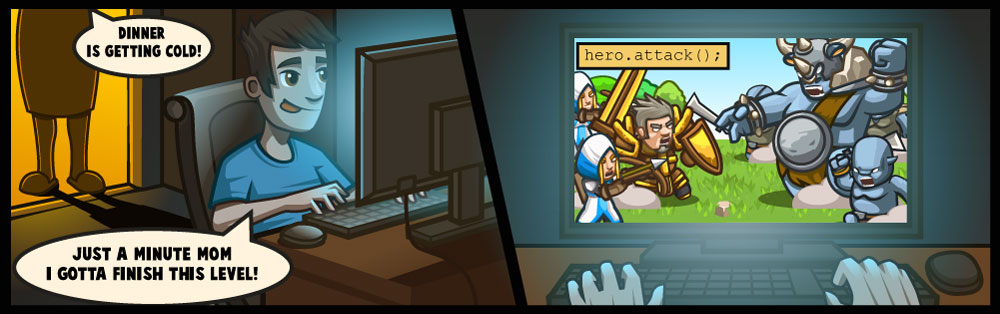
\includegraphics[width=\textwidth]{images/about_comic.jpg}\\
    \textbf Playing the Game
    \begin{itemize}
    \item Start by Picking a Language
    \item Each "Dungeon" teaches different programming fundamentals
    \end{itemize}
\end{frame}

\begin{frame}{The Game}
    \href{http://codecombat.com/cla}{CodeCombat Individual CLA}
    \begin{itemize}
    \item You retain your rights both to Copyright and Patents
    \item Also grant rights to both Copyright and Patents to CodeCombat
    \end{itemize}
\end{frame}

\section{Contributing}

\begin{frame}{How to get involved}
    \centerline{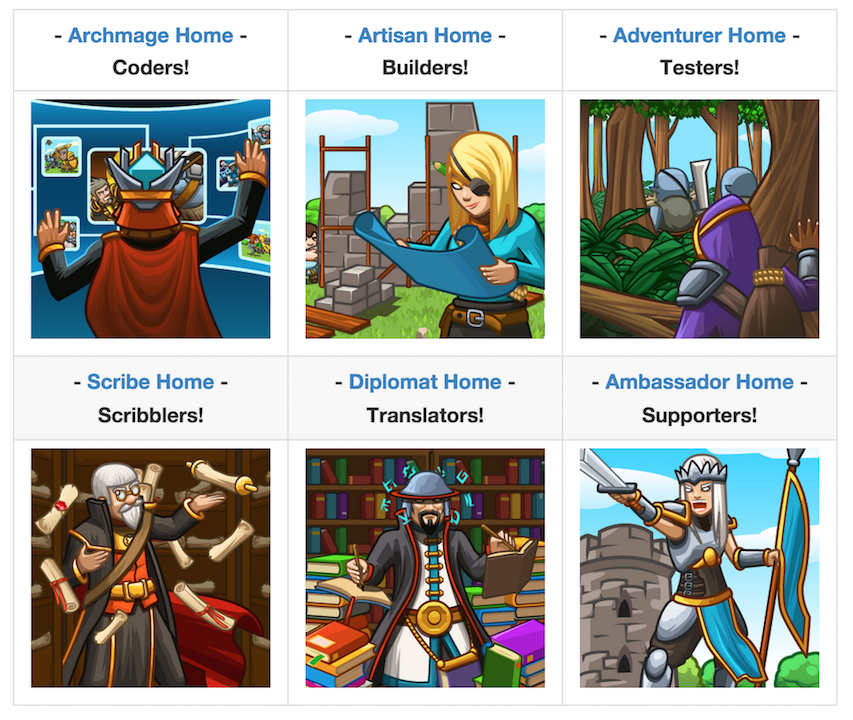
\includegraphics[width=\textwidth,height=8cm, keepaspectratio]{images/getinvolved.png}}
\end{frame}

\begin{frame}{Patches}
   \centerline{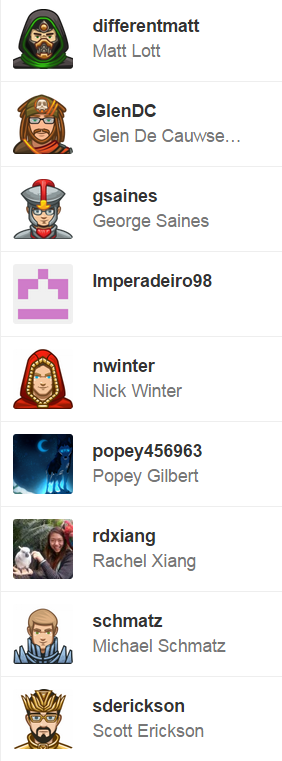
\includegraphics[width=\textwidth, height=8cm, keepaspectratio]{images/close.png}}
    
\end{frame}

\begin{frame}{Group Process}
    \begin{itemize}
    \item Barely contained chaos, over 200 open issues. 300+ contributers
    \item Participation trending up
    \item Really good getting involved process, lots of documentation
    \end{itemize}
    
\end{frame}

\begin{frame}{Git by a Bus / Raptor}
    \begin{itemize}
    \item Git by a Bus - Probably not. the most active 20 percent are people who are employed to create this game. 
    \item Raptor - Hopefully. There is more than one very active committer. 
    \centerline{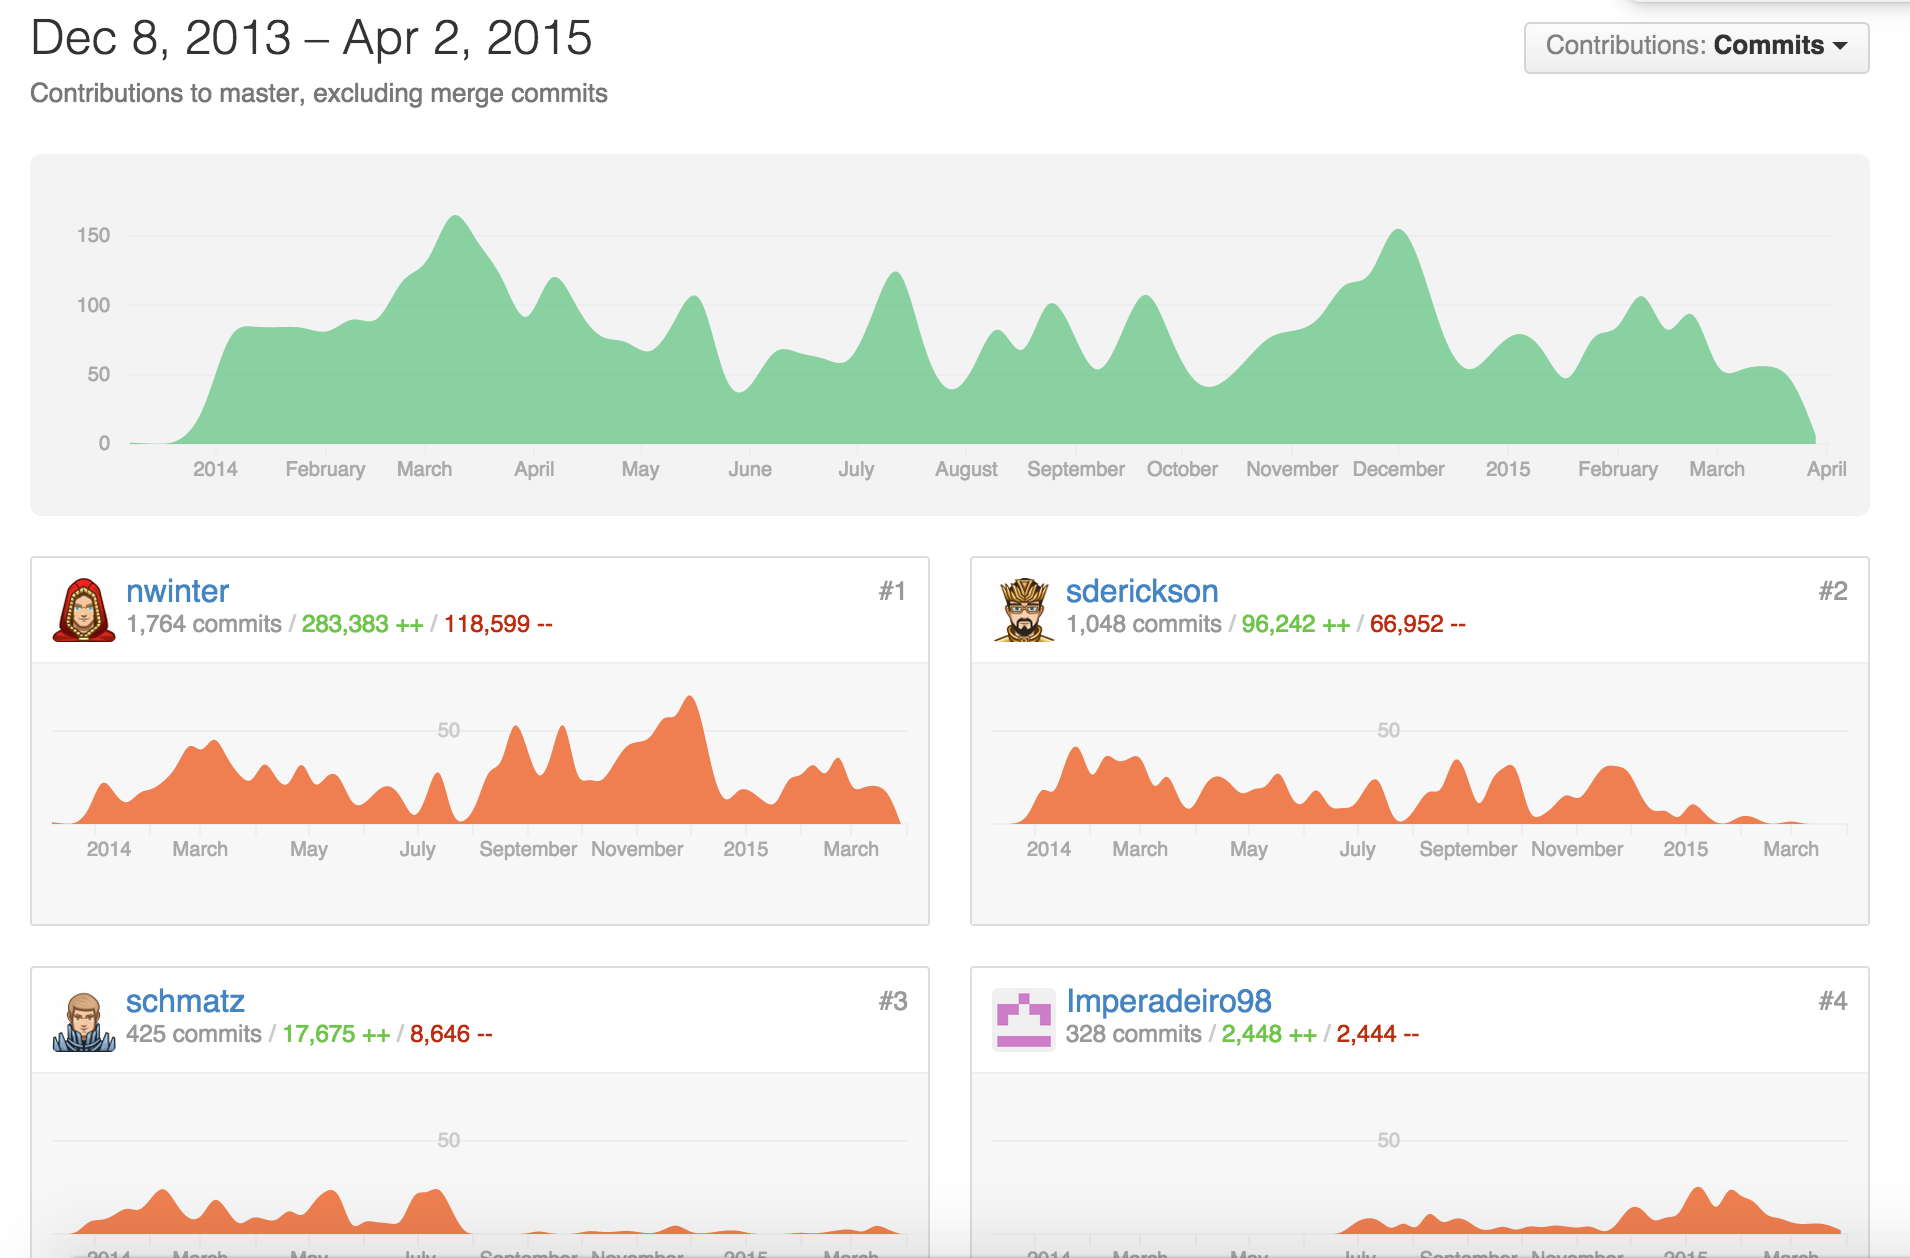
\includegraphics[width=\textwidth, height=5cm, keepaspectratio]{images/graph.png}}
    
    \end{itemize}
    
\end{frame}

\begin{frame}{Summary}

  Get the source of this theme and the demo presentation from

  \begin{center}\url{github.com/matze/mtheme}\end{center}

  The theme \emph{itself} is licensed under a
  \href{http://creativecommons.org/licenses/by-sa/4.0/}{Creative Commons
  Attribution-ShareAlike 4.0 International License}.

  \begin{center}\ccbysa\end{center}

\end{frame}

\plain{}{Questions?}

\end{document}
